\documentclass{beamer}
% Some basic packagesLLuu
\usepackage[utf8]{inputenc}
\usepackage{spverbatim}
\usepackage{textcomp}
\usepackage{pgfplots}
\usepackage{url}
\usepackage{graphicx}
\usepackage{float}
\usepackage{algorithm2e}
\usepackage{enumitem}
\usepackage{standalone}
\usepackage{tcolorbox}
\usepackage{wrapfig}
% \usepackage{svg}
% \usepackage{svg-inkscape} 

\graphicspath{{./figures}}

%color settings
\usepackage{xcolor}
\definecolor{gruvbgdark}{HTML}{1d2021}
\definecolor{gruvtextdark}{HTML}{ebdbb2}
\definecolor{gruvbglight}{HTML}{f9f5d7}
\definecolor{gruvtextlight}{HTML}{3c3836}
\definecolor{NavyBlue}{HTML}{266bbd}
\definecolor{RawSienna}{HTML}{94330e}
\definecolor{ForestGreen}{HTML}{149b52}
% \pagecolor{gruvbgdark}
% \color{gruvtextdark}

% Hide page number when page is empty
\usepackage{emptypage}
\usepackage{subcaption}
\usepackage{multicol}

% Math stuff
\usepackage{amsmath, amsfonts, mathtools, amsthm, amssymb}
% Fancy script capitals
\usepackage{mathrsfs}
\usepackage{cancel}

% Bold math
\usepackage{bm}

%Algorithm setup
\RestyleAlgo{algoruled}
% Some shortcuts
\newcommand\N{\ensuremath{\mathbb{N}}}
\newcommand\R{\ensuremath{\mathbb{R}}}
\newcommand\Z{\ensuremath{\mathbb{Z}}}
\renewcommand\O{\ensuremath{\emptyset}}
\newcommand\Q{\ensuremath{\mathbb{Q}}}
\newcommand\C{\ensuremath{\mathbb{C}}}
\newcommand\B{\ensuremath{\mathbb{B}}}

%Make implies and impliedby shorter
\let\implies\Rightarrow
\let\impliedby\Leftarrow
\let\iff\Leftrightarrow

\let\epsilon\varepsilon

% Add \contra symbol to denote contradiction
% \usepackage{stmaryrd} % for \lightning
% \newcommand\contra{\scalebox{1.5}{$\lightning$}}

\let\phi\varphi

% Command for short corrections
% Usage: 1+1=\correct{3}{2}

\definecolor{correct}{HTML}{009900}
\newcommand\correct[2]{\ensuremath{\:}{\color{red}{#1}}\ensuremath{\to }{\color{correct}{#2}}\ensuremath{\:}}
\newcommand\green[1]{{\color{correct}{#1}}}

% horizontal rule
% \newcommand\hr{
%     \noindent\rule[0.5ex]{\linewidth}{0.5pt}
% }

% hide parts
\newcommand\hide[1]{}

% Environments
\makeatother


\newcommand{\oefening}[1]{%
	\def\@oefening{#1}%
	\subsection*{Oefening #1}
}

\newcommand{\suboefening}[1]{%
	\subsubsection*{Oefening \@oefening.#1}
}


% \lecture starts a new lecture (les in dutch)
%
% Usage:
% \lecture{1}{di 12 feb 2019 16:00}{Inleiding}
%
% This adds a section heading with the number / title of the lecture and a
% margin paragraph with the date.

% I use \dateparts here to hide the year (2019). This way, I can easily parse
% the date of each lecture unambiguously while still having a human-friendly
% short format printed to the pdf.

% \usepackage{xifthen}
% \def\testdateparts#1{\dateparts#1\relax}
% \def\dateparts#1 #2 #3 #4 #5\relax{
% 	\marginpar{\small\textsf{\mbox{#1 #2 #3 #5}}}
% }

% \def\@lecture{}%
% \newcommand{\lecture}[3]{
% 	\ifthenelse{\isempty{#3}}{%
% 		\def\@lecture{Lecture #1}%
% 	}{%
% 		\def\@lecture{Lecture #1: #3}%
% 	}%
% 	\subsection*{\@lecture}
% 	% \marginpar{\small\textsf{\mbox{#2}}}
% }

\usepackage{listings}

\definecolor{dkgreen}{rgb}{0,0.6,0}
\definecolor{gray}{rgb}{0.5,0.5,0.5}
\definecolor{mauve}{rgb}{0.58,0,0.82}

\lstset{frame=none,
  language=python,
  aboveskip=3mm,
  belowskip=3mm,
  showstringspaces=false,
  columns=flexible,
  basicstyle={\small\ttfamily},
  numbers=none,
  numberstyle=\tiny\color{gray},
  keywordstyle=\color{blue},
  commentstyle=\color{dkgreen},
  stringstyle=\color{mauve},
  breaklines=true,
  breakatwhitespace=true,
  tabsize=3
}



% These are the fancy headers

% LE: left even
% RO: right odd
% CE, CO: center even, center odd
% My name for when I print my lecture notes to use for an open book exam.

\makeatother

\usepackage{tcolorbox}

% Make boxes breakable
\tcbuselibrary{breakable}

% Figure support as explained in my blog post.
\usepackage{import}
\usepackage{xifthen}
\usepackage{pdfpages}
\usepackage{transparent}
\newcommand{\incfig}[2][1]{%
	% \begin{center}
	\def\svgwidth{#1\columnwidth}
	\import{./figures/}{#2.pdf_tex}
	% \end{center}
}
% Fix some stuff
% %http://tex.stackexchange.com/questions/76273/multiple-pdfs-with-page-group-included-in-a-single-page-warning
\pdfsuppresswarningpagegroup=1
\author{Kristian Sørdal}

%Information to be included in the title page:
\title{CSR SPMV - Results}
\author{Kristian Sørdal}
\institute{University of Bergen}

\begin{document}

\frame{\titlepage}

\begin{frame}
\frametitle{Shared Memory Total Time - fpgaq}
\begin{figure}
  \centering

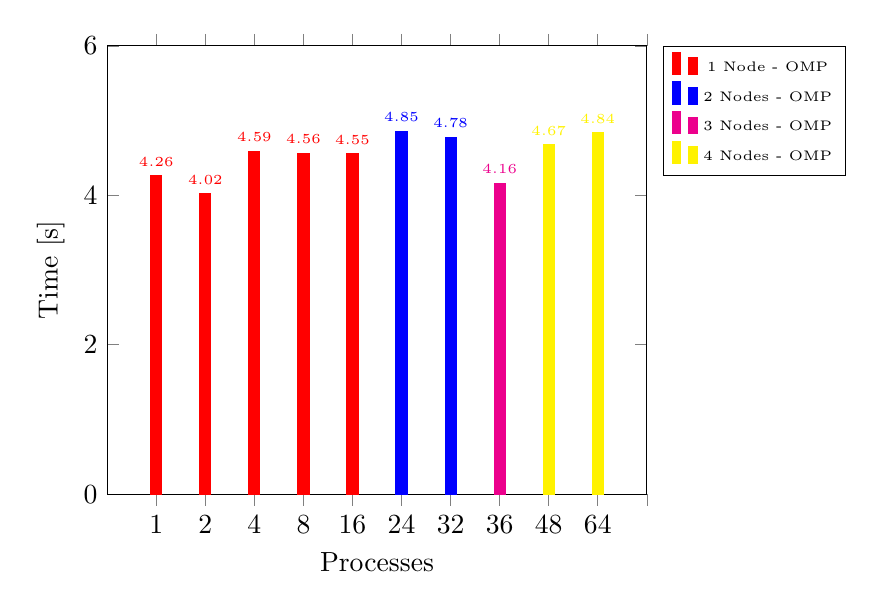
\begin{tikzpicture}
  \begin{axis}[
    xlabel={Processes},
    ylabel={Time [s]},
    legend pos=outer north east,
    legend style={font=\tiny},
    ymin = 0, ymax = 6,
    xmin = 0, xmax = 11,
    % xmode=log,
    xtick={1,2,3,4,5,6,7,8,9,10,11},
    xticklabels={1,2,4,8,16,24,32,36,48,64},
    ybar,
    bar width=4pt,
    bar shift = 0mm,
    xscale=1,
    nodes near coords,
    nodes near coords style={font=\tiny}
    ]
    % Bar 1
    \addplot[red, fill=red] coordinates {
            (1,4.2583)
            (2,4.01827)
            (3,4.58939)
            (4,4.56112)
            (5,4.55471)
    };
    \addlegendentry{1 Node - OMP}
    \addplot[blue, fill=blue] coordinates {
            (6,4.85173)
            (7,4.77806)
    };
    \addlegendentry{2 Nodes - OMP}
    \addplot[magenta, fill=magenta] coordinates {
            (8,4.15607)
    };
    \addlegendentry{3 Nodes - OMP}
    \addplot[yellow, fill=yellow] coordinates {
            (9,4.67419)
            (10,4.83562)
    };
    \addlegendentry{4 Nodes - OMP}
    
  \end{axis}
\end{tikzpicture}
\end{figure}
\end{frame}
\begin{frame}
\frametitle{Distributed Memory Total Time - fpgaq}
\begin{figure}
  \centering

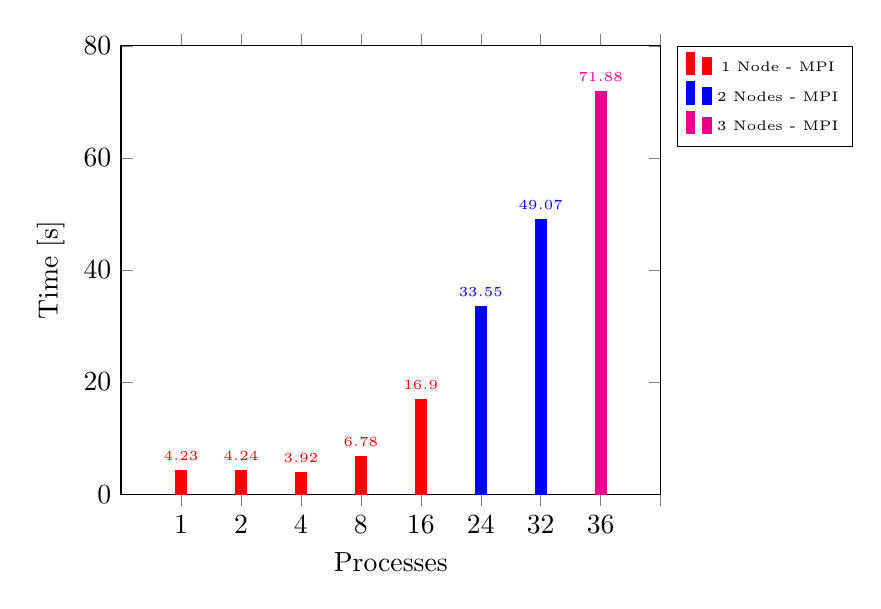
\begin{tikzpicture}
  \begin{axis}[
    xlabel={Processes},
    ylabel={Time [s]},
    legend pos=outer north east,
    legend style={font=\tiny},
    ymin = 0, ymax = 80,
    xmin = 0, xmax = 9,
    % xmode=log,
    xtick={1,2,3,4,5,6,7,8,9},
    xticklabels={1,2,4,8,16,24,32,36},
    ybar,
    bar width=4pt,
    bar shift = 0mm,
    xscale=1,
    nodes near coords,
    nodes near coords style={font=\tiny}
    ]
    \addplot[red, fill=red] coordinates {
            (1,4.22763)
            (2,4.24122)
            (3,3.9193)
            (4,6.77588)
            (5,16.9037)
    };
    \addlegendentry{1 Node - MPI}
    \addplot[blue, fill=blue] coordinates {
            (6,33.5535)
            (7,49.0719)
    };
    \addlegendentry{2 Nodes - MPI}
    \addplot[magenta, fill=magenta] coordinates {
            (8,71.878)
    };
    \addlegendentry{3 Nodes - MPI}
  \end{axis}
\end{tikzpicture}
\end{figure}
\end{frame}
\begin{frame}
\frametitle{Shared Memory GFLOPS - fpgaq}
\begin{figure}
  \centering

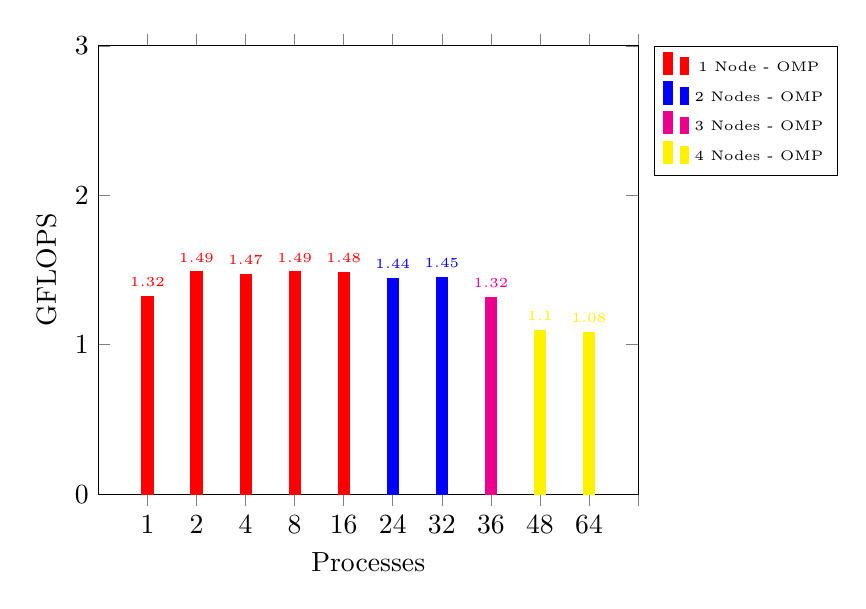
\begin{tikzpicture}
  \begin{axis}[
    xlabel={Processes},
    ylabel={GFLOPS},
    legend pos=outer north east,
    legend style={font=\tiny},
    ymin = 0, ymax = 3,
    xmin = 0, xmax = 11,
    % xmode=log,
    xtick={1,2,3,4,5,6,7,8,9,10,11},
    xticklabels={1,2,4,8,16,24,32,36,48,64},
    ybar,
    bar width=4pt,
    bar shift = 0mm,
    xscale=1,
    nodes near coords,
    nodes near coords style={font=\tiny}
    ]
    % Bar 1
    \addplot[red, fill=red] coordinates {
            (1,1.32331)
            (2,1.48745)
            (3,1.46831)
            (4,1.48671)
            (5,1.48255)
    };
    \addlegendentry{1 Node - OMP}
    \addplot[blue, fill=blue] coordinates {
            (6,1.44259)
            (7,1.45192)
    };
    \addlegendentry{2 Nodes - OMP}
    \addplot[magenta, fill=magenta] coordinates {
            (8,1.31552)
    };
    \addlegendentry{3 Nodes - OMP}
    \addplot[yellow, fill=yellow] coordinates {
            (9,1.09636)
            (10,1.08321)
    };
    \addlegendentry{4 Nodes - OMP}
    
  \end{axis}
\end{tikzpicture}
\end{figure}
\end{frame}
\begin{frame}
\frametitle{Shared Memory GFLOPS (Kernel) - fpgaq}
\begin{figure}
  \centering

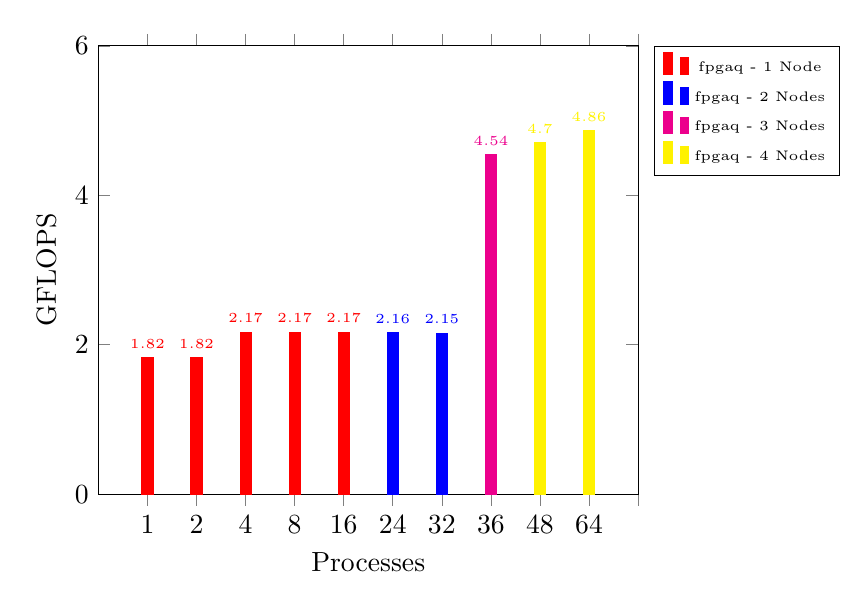
\begin{tikzpicture}
  \begin{axis}[
    xlabel={Processes},
    ylabel={GFLOPS},
    legend pos=outer north east,
    legend style={font=\tiny},
    ymin = 0, ymax = 6,
    xmin = 0, xmax = 11,
    % xmode=log,
    xtick={1,2,3,4,5,6,7,8,9,10,11},
    xticklabels={1,2,4,8,16,24,32,36,48,64},
    ybar,
    bar width=4pt,
    bar shift = 0mm,
    xscale=1,
    nodes near coords,
    nodes near coords style={font=\tiny}
    ]
    % Bar 1
    \addplot[red, fill=red] coordinates {
            (1,1.82264)
            (2,1.82264)
            (3,2.16646)
            (4,2.16646)
            (5,2.16646)
    };
    \addlegendentry{fpgaq - 1 Node}
    \addplot[blue, fill=blue] coordinates {
            (6,2.15803)
            (7,2.15027)
    };
    \addlegendentry{fpgaq - 2 Nodes}
    \addplot[magenta, fill=magenta] coordinates {
            (8,4.53922)
    };
    \addlegendentry{fpgaq - 3 Nodes}
    \addplot[yellow, fill=yellow] coordinates {
            (9,4.7021)
            (10,4.86267)
    };
    \addlegendentry{fpgaq - 4 Nodes}
    
  \end{axis}
\end{tikzpicture}
\end{figure}
\end{frame}
\begin{frame}
\frametitle{Distributed Memory GFLOPS - fpgaq}
\begin{figure}
  \centering

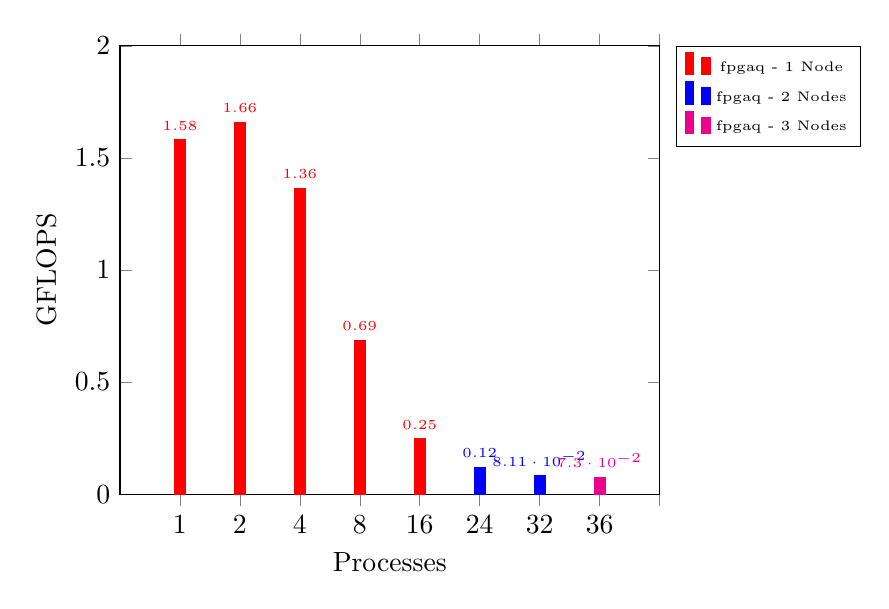
\begin{tikzpicture}
  \begin{axis}[
    xlabel={Processes},
    ylabel={GFLOPS},
    legend pos=outer north east,
    legend style={font=\tiny},
    ymin = 0, ymax = 2,
    xmin = 0, xmax = 9,
    % xmode=log,
    xtick={1,2,3,4,5,6,7,8,9},
    xticklabels={1,2,4,8,16,24,32,36},
    ybar,
    bar width=4pt,
    bar shift = 0mm,
    xscale=1,
    nodes near coords,
    nodes near coords style={font=\tiny}
    ]
    % Bar 1
    \addplot[red, fill=red] coordinates {
            (1,1.58074)
            (2,1.65778)
            (3,1.36284)
            (4,0.687124)
            (5,0.246568)
    };
    \addlegendentry{fpgaq - 1 Node}
    \addplot[blue, fill=blue] coordinates {
            (6,0.11978)
            (7,0.0810677)
    };
    \addlegendentry{fpgaq - 2 Nodes}
    \addplot[magenta, fill=magenta] coordinates {
            (8,0.0730397)
    };
    \addlegendentry{fpgaq - 3 Nodes}
    
  \end{axis}
\end{tikzpicture}
\end{figure}
\end{frame}
\begin{frame}
\frametitle{Distributed Memory GFLOPS (kernel) - fpgaq}
\begin{figure}
  \centering

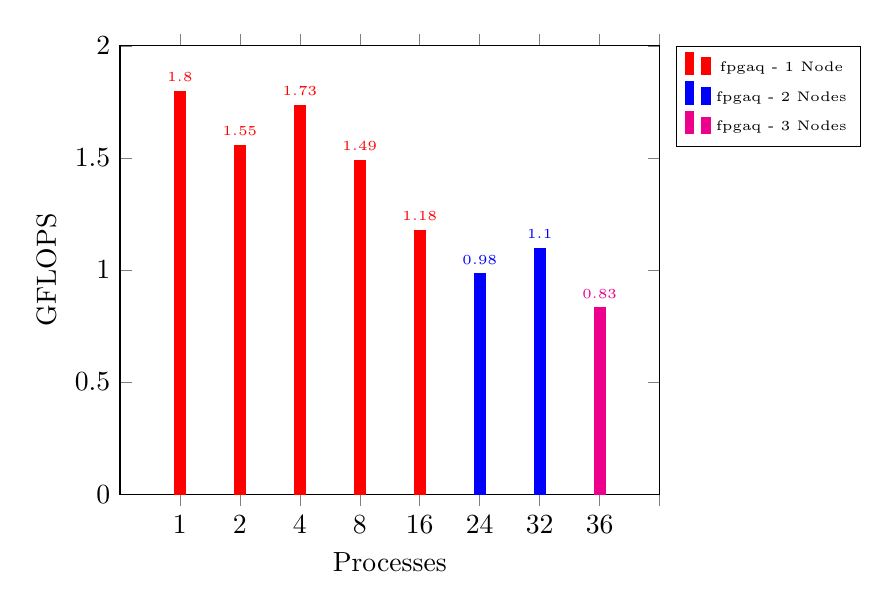
\begin{tikzpicture}
  \begin{axis}[
    xlabel={Processes},
    ylabel={GFLOPS},
    legend pos=outer north east,
    legend style={font=\tiny},
    ymin = 0, ymax = 2,
    xmin = 0, xmax = 9,
    % xmode=log,
    xtick={1,2,3,4,5,6,7,8,9},
    xticklabels={1,2,4,8,16,24,32,36},
    ybar,
    bar width=4pt,
    bar shift = 0mm,
    xscale=1,
    nodes near coords,
    nodes near coords style={font=\tiny}
    ]
    % Bar 1
    \addplot[red, fill=red] coordinates {
            (1,1.79702)
            (2,1.55414)
            (3,1.73431)
            (4,1.488)
            (5,1.17592)
    };
    \addlegendentry{fpgaq - 1 Node}
    \addplot[blue, fill=blue] coordinates {
            (6,0.982533)
            (7,1.09548)
    };
    \addlegendentry{fpgaq - 2 Nodes}
    \addplot[magenta, fill=magenta] coordinates {
            (8,0.830298)
    };
    \addlegendentry{fpgaq - 3 Nodes}
    
  \end{axis}
\end{tikzpicture}
\end{figure}
\end{frame}
\begin{frame}
\frametitle{Distributed Memory Communication Time  - fpgaq}
\begin{figure}
  \centering

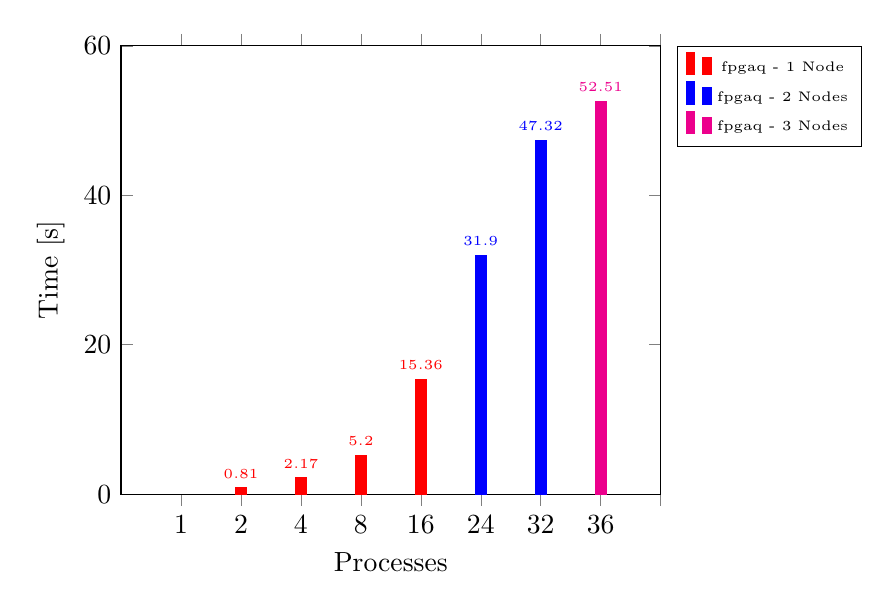
\begin{tikzpicture}
  \begin{axis}[
    xlabel={Processes},
    ylabel={Time [s]},
    legend pos=outer north east,
    legend style={font=\tiny},
    ymin = 0, ymax = 60,
    xmin = 0, xmax = 9,
    % xmode=log,
    xtick={1,2,3,4,5,6,7,8,9},
    xticklabels={1,2,4,8,16,24,32,36},
    ybar,
    bar width=4pt,
    bar shift = 0mm,
    xscale=1,
    nodes near coords,
    nodes near coords style={font=\tiny}
    ]
    % Bar 1
    \addplot[red, fill=red] coordinates {
            (2,0.81438)
            (3,2.17099)
            (4,5.19863)
            (5,15.3598)
    };
    \addlegendentry{fpgaq - 1 Node}
    \addplot[blue, fill=blue] coordinates {
            (6,31.9033)
            (7,47.3188)
    };
    \addlegendentry{fpgaq - 2 Nodes}
    \addplot[magenta, fill=magenta] coordinates {
            (8,52.5106)
    };
    \addlegendentry{fpgaq - 3 Nodes}
    
  \end{axis}
\end{tikzpicture}
\end{figure}
\end{frame}
\end{document}

